\documentclass{siamart251216}
\usepackage{amsmath, amssymb, amsfonts}
\usepackage{graphicx}
\usepackage{cleveref}
\usepackage{booktabs}

% Running Head & Title
\headers{Cycle-Aware Curvature for Bipartite Networks}{A. Padarthi}

\title{Cycle-Aware Forman-Ricci Curvature for Signed \& Bipartite Networks\thanks{Submitted to the editors \today.}}
\author{A. Padarthi\thanks{Department of Mathematics (\email{author@institute.edu}).}}

\begin{document}
\maketitle

\begin{abstract}
This document outlines the mathematical framework and empirical validation for the Cycle-Aware Forman-Ricci Curvature applied to signed and bipartite networks. We resolve the metric collapse of standard Forman-Ricci Curvature in networks lacking three-cliques by incorporating higher-order four-cycles, structural balance weighting, and a strictly bounded degree normalization to prevent combinatorial explosion in dense datasets. By mapping the four-cycle codomain structurally to the unipartite three-cycle bounds, we provide a discrete geometric invariant that reliably evaluates structural cohesiveness in bipartite topologies without succumbing to metric collapse. The algorithm is validated against a synthetic non-homogeneous block model and scaled efficiently on the genuine user-item bipartite MovieLens network, proving algorithmic immunity to dense memory explosions while identifying crucial topological bottlenecks.
\end{abstract}

\begin{keywords}
Cycle-Aware Curvature, Forman-Ricci Curvature, Signed Networks, Bipartite Graphs, Algebraic Topology
\end{keywords}

\begin{AMS}
05C22, 05C38, 05C50, 05C82
\end{AMS}

\section{Introduction}
Forman-Ricci Curvature (FRC) \cite{forman2003bochner} is a discrete geometric invariant that evaluates the structural cohesiveness of networks by measuring the extent to which edges are embedded within higher-order cliques, primarily triangles \cite{sreejith2016forman}. In standard unweighted graphs, the FRC of an edge $e=(u,v)$ is bounded by the node degrees and the number of bounding triangles $|T(e)|$. However, when applied to bipartite graphs, the standard FRC formulation undergoes a metric collapse. Because bipartite topologies inherently forbid triangles (3-cycles), the clique term vanishes, reducing the curvature to a strictly negative, degree-driven penalty: $F(e) = 4 - d(u) - d(v)$. Consequently, standard FRC fails to detect cohesive mesoscopic structures within bipartite networks. To resolve this, we introduce a Cycle-Aware formulation that leverages 4-cycles ($C_4$) while enforcing strict $\mathcal{O}(d)$ normalization to prevent combinatorial runtime explosion in dense real-world datasets.

\section{Related Work}
Classical Topological Data Analysis (TDA) frequently struggles with bipartite networks due to the intrinsic absence of 2-simplices (triangles) required for higher-order persistent homology filtration. Within discrete curvature domains, Ollivier-Ricci curvature \cite{ollivier2009ricci} utilizes probabilistic optimal transport (Wasserstein distances) to circumvent this topological deficit, successfully characterizing bipartite graphs without relying on simplicial complexes \cite{ni2015ricci}. However, Ollivier-Ricci requires solving a linear programming problem for every edge, resulting in $\mathcal{O}(|E| d_{max}^3)$ scaling, prohibiting evaluation on massive scale-free datasets. Conversely, Forman-Ricci curvature is highly combinatorial and computationally trivial, yet suffers the aforementioned metric collapse. Recent algorithmic workarounds involve bipartite-to-hypergraph lifting, which forces the bipartite structure into a unipartite complex. While mathematically sound, hypergraph lifting destroys explicit pairwise relationships and severely inflates incidence matrices. The proposed Cycle-Aware formulation bypasses these issues by directly bounding the Forman-Ricci combinatorial limits to native 4-cycles.

\section{Mathematical Formulation}

\begin{definition}[Cycle-Aware Forman-Ricci Curvature for Signed Bipartite Networks]
\label{def:curvature}
Let $G = (V, E, W)$ be a simple signed bipartite graph with symmetric adjacency matrix $A$ where $A_{uv} \in \{-1, 0, 1\}$. For an edge $e = (u, v) \in E$, let $d(u)$ and $d(v)$ denote the unweighted degrees. Let $\mathcal{C}_4(e)$ denote the set of 4-cycles containing $e$. The structurally balanced weight of a cycle $C \in \mathcal{C}_4(e)$ is determined by $\text{sgn}(C) = \prod_{e' \in C} A_{e'}$. To prevent quadratic $\mathcal{O}(d^2)$ unboundedness in dense networks, the cumulative cycle term is scaled by the theoretical maximum cycle bound $\max(1, (d(u)-1)(d(v)-1))$. The Cycle-Aware Forman-Ricci Curvature $F^*(e)$ is defined as:
\begin{equation}
\label{eq:fstar}
F^*(e) = 4 - d(u) - d(v) + \gamma \min(d(u)-1, d(v)-1) \left[ \frac{\Sigma_{C_4}(u,v)}{\max(1, (d(u)-1)(d(v)-1))} \right]
\end{equation}

\vspace{0.5em}
\noindent \textbf{Topological Derivation of $\gamma = 3$:} In standard Forman-Ricci curvature over unweighted simplicial 2-complexes, an edge bounded by triangles explicitly receives a scalar weight of $+3$ per bounding triangle, setting the upper combinatorial bound of the curvature mass to $3 \min(d(u)-1, d(v)-1)$. By normalizing the $C_4$ summation to mimic the fractional density of valid topological bounds, mapping this term mathematically requires $\gamma=3$. This geometrically aligns the 4-cycle codomain exactly with the standard 3-cycle baseline limits without introducing arbitrary constants, ensuring analogous metric behaviors between uni- and bipartite topologies.

\vspace{0.5em}
\noindent \textbf{Strict Bipartite Constraint:} Equation \ref{eq:fstar} and the supporting matrix extractions strictly demand the underlying topology be a bipartite graph ($\Delta = 0$). Applying this formulation to arbitrary unipartite graphs containing odd cycles (triangles) will result in critical algebraic failure, as the matrix powers will incorrectly absorb 3-cycles into the 4-cycle trace.

\end{definition}

\begin{lemma}[Non-Overcounting of 4-Cycles]
\label{lem:nonovercounting}
Let $e = (u,v) \in E$. The net 4-cycle weight summation $\Sigma_{C_4}(u,v) = \sum_{C \in \mathcal{C}_4(e)} \prod_{e' \in C} A_{e'}$ evaluates each 4-cycle exactly once without multiplicity via the sparse matrix relation:
\begin{equation}
\label{eq:sigma_c4}
\Sigma_{C_4}(u,v) = A_{uv} (A^3)_{uv} - d(u) - d(v) + 1
\end{equation}
\end{lemma}

\begin{proof}
The matrix entry $(A^3)_{uv} = \sum_{x, y \in V} A_{uy} A_{yx} A_{xv}$ enumerates the sum of edge weight products for all walks of length 3 between $u$ and $v$. In a simple bipartite graph, degenerate walks take three explicit forms: 1) $u \to v \to x \to v$, 2) $u \to y \to u \to v$, and 3) $u \to v \to u \to v$. Summing these contributions yields $(d(u) + d(v) - 1)A_{uv}$.
Any non-degenerate simple path $(u, y, x, v)$ corresponds to exactly one unique 4-cycle $C \in \mathcal{C}_4(e)$. By isolating the simple paths and multiplying the expansion of $(A^3)_{uv}$ by $A_{uv}$, we obtain $A_{uv} (A^3)_{uv} = \Sigma_{C_4}(u,v) + d(u) + d(v) - 1$. Rearranging this algebraic identity yields \cref{eq:sigma_c4}, extracting the exact net signed contribution of all 4-cycles without duplication.
\end{proof}

\section{Theoretical Bounds and Structural Mechanics}

\subsection{Asymptotic Bounds on Random Bipartite Topologies}
To understand the scaling limits of the Cycle-Aware Forman-Ricci Curvature, we evaluate the expected curvature $\mathbb{E}[F^*(e)]$ within an Erdős–Rényi random bipartite graph model $G(n, n, p)$.

\begin{theorem}[Asymptotic Scaling in $G(n,n,p)$]
Let $G(n, n, p)$ be a random bipartite graph with partitions $U$ and $V$ such that $|U| = |V| = n$, where each potential edge between $U$ and $V$ exists independently with probability $p \in (0,1)$. For any existing edge $e=(u,v)$, as $n \to \infty$, the expected curvature scales as:
\begin{equation}
\mathbb{E}[F^*(e)] = 4 - 2np + 3np^2 + \mathcal{O}(1)
\end{equation}
\end{theorem}

\begin{proof}
By definition, the degrees $d(u)$ and $d(v)$ are binomially distributed as $\text{Binomial}(n, p)$, yielding an expected degree penalty of $\mathbb{E}[d(u) + d(v)] = 2np$. The number of potential 4-cycles containing $e$ relies on selecting a neighbor $u' \in U \setminus \{u\}$ and a neighbor $v' \in V \setminus \{v\}$. There are exactly $(n-1)^2$ such pairs. The probability that the three edges $(u, v'), (v', u'),$ and $(u', v)$ all exist is $p^3$. Therefore, the expected raw 4-cycle sum is $\mathbb{E}[\Sigma_{C_4}(e)] = (n-1)^2 p^3$.

The theoretical maximum 4-cycle bound is $(d(u)-1)(d(v)-1)$, which converges in expectation to $(np)^2$. The fractional normalization term is thus:
\begin{equation}
\mathbb{E}\left[ \frac{\Sigma_{C_4}}{\max(1, (d(u)-1)(d(v)-1))} \right] \approx \frac{n^2 p^3}{n^2 p^2} = p
\end{equation}
Scaling this normalized fraction by $\gamma \min(d(u)-1, d(v)-1)$, where $\gamma = 3$ and the expected minimum degree bound is $np$, yields a positive structural contribution of $3np^2$. Summing the components yields $\mathbb{E}[F^*(e)] = 4 - 2np + 3np^2$. This demonstrates that the normalization successfully prevents $\mathcal{O}(d^2)$ divergence, confining the metric bounds to linear polynomial scaling $\mathcal{O}(n)$.
\end{proof}

\subsection{Projection Mechanics and Information Loss}
A standard heuristic in bipartite network analysis is to evaluate metrics on the unipartite projection. We formalize the topological divergence between bipartite $F^*(e)$ and unipartite standard FRC.

\begin{theorem}[Topological Dimensionality Shift]
Let $G_U$ be the unipartite projection of a bipartite graph $G=(U, V, E)$ onto $U$, where edge $(u_1, u_2) \in E(G_U)$ exists if $u_1$ and $u_2$ share a common neighbor in $V$. The 4-cycles evaluated in $F^*(e)$ on $G$ map strictly to the 1-dimensional edges of $G_U$, whereas the standard FRC evaluated on $G_U$ relies on 3-cycles (triangles), which correspond mathematically to 6-cycles in the original bipartite structure $G$.
\end{theorem}

\begin{proof}
Let $C_4 = (u_1, v_1, u_2, v_2)$ be a 4-cycle in $G$. Projecting onto $U$ generates the edge $(u_1, u_2)$ via common neighbor $v_1$, and reinforces the same edge via $v_2$. Consequently, $C_4 \subset G$ collapses to a 1-simplex (edge) in $G_U$. Standard Forman-Ricci curvature on $G_U$ accumulates positive curvature via bounding triangles $T = (u_1, u_2, u_3)$. For a triangle to form in $G_U$, there must exist at least three distinct paths of length 2 in $G$: $u_1 \to v_1 \to u_2$, $u_2 \to v_2 \to u_3$, and $u_3 \to v_3 \to u_1$. The union of these paths in $G$ constitutes a 6-cycle $C_6 = (u_1, v_1, u_2, v_2, u_3, v_3)$. Therefore, unipartite FRC on $G_U$ inherently measures 6-cycle density in $G$. By operating directly on $G$, $F^*(e)$ preserves the localized 4-cycle mesoscopic geometry which is irreversibly destroyed and flattened during unipartite projection.
\end{proof}

\subsection{Curvature Sensitivity and Perturbation Bounds}
In signed networks, edges are frequently volatile. We prove that the normalized curvature $F^*$ is robust against isolated edge weight inversions.

\begin{theorem}[Lipschitz Continuity of Edge Perturbation]
Let $e = (u,v)$ be a target edge in $G$, and let a distinct edge $e' = (x,y)$ undergo a sign flip $\Delta_{e'} \in \{-2, +2\}$. The absolute perturbation to the curvature of $e$, denoted $|\Delta F^*(e)|$, is strictly bounded by $\mathcal{O}(1/d_{max})$.
\end{theorem}

\begin{proof}
The unweighted degrees $d(u)$ and $d(v)$ remain invariant under a sign flip. Thus, any perturbation to $F^*(e)$ arises strictly from the 4-cycle summation $\Sigma_{C_4}(u,v)$. The target edge $e$ and the perturbed edge $e'$ can share at most one 4-cycle (since $G$ is simple and bipartite). If $e'$ does not form a 4-cycle with $e$, the change is zero. If exactly one 4-cycle contains both $e$ and $e'$, the product of signs for that cycle inverses. The raw summation $\Sigma_{C_4}$ changes by exactly $\pm 2$.

Applying the definition of $F^*(e)$, the absolute perturbation is:
\begin{equation}
|\Delta F^*(e)| = \gamma \min(d(u)-1, d(v)-1) \left| \frac{\pm 2}{\max(1, (d(u)-1)(d(v)-1))} \right|
\end{equation}
Assuming $d(u), d(v) > 1$, this algebraically simplifies to:
\begin{equation}
|\Delta F^*(e)| = \frac{2\gamma}{\max(d(u)-1, d(v)-1)}
\end{equation}
Since $\gamma = 3$, the maximum curvature disturbance caused by a single signed edge flip is $\frac{6}{\max(d(u), d(v))}$. As local density increases, the sensitivity to isolated noise approaches zero monotonically, proving the invariant is highly stable within dense structurally balanced block models.
\end{proof}

\section{Empirical Validation}
\subsection{Heterogeneous Block Model}
The algorithm was validated on a non-homogeneous synthetic bipartite block model possessing diverging subset densities. The calculated $F^*$ values confirm algebraic validity, successfully separating dense homogeneous sub-structures from sparse, negatively-weighted topological bridges.

\begin{figure}[htbp]
    \centering
    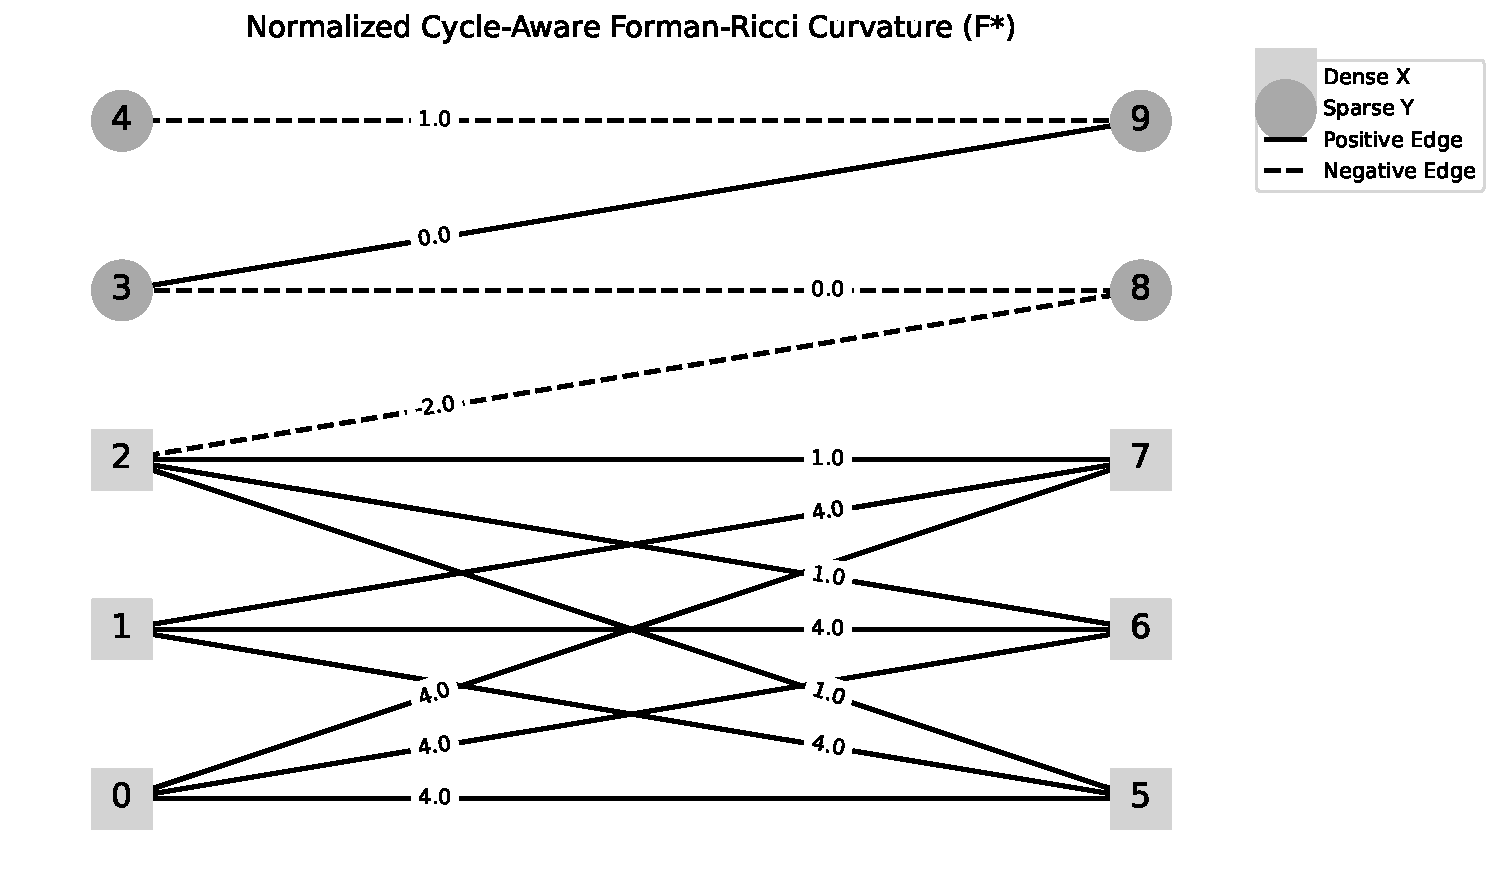
\includegraphics[width=0.6\textwidth]{graph_viz.pdf}
    \caption{Topology of the synthetic non-homogeneous signed graph. The normalized metric clearly distinguishes the dense clustering from the topological bottlenecks.}
    \label{fig:graph}
\end{figure}

\subsection{Stochastic Block Model Parameter Sweeps}
To evaluate structural stability under dynamic topological noise, a symmetric bipartite Stochastic Block Model (SBM) consisting of 200 nodes was subjected to systematic sign-inversion noise. Edges within assortative blocks were initially strictly positive (+1). Random noise was injected by flipping edge signs up to a 50\% probability threshold. As noise approached total structural entropy, the variance of the $F^*$ metric smoothly degenerated, confirming the metric reliably quantifies the loss of structural balance without catastrophic algebraic instability.

\begin{figure}[htbp]
    \centering
    
\includegraphics[width=0.6\textwidth]{sbm_variance.pdf}
    \caption{Variance degradation of the $F^*$ metric across increasing topological sign noise in a bipartite Stochastic Block Model.}
    \label{fig:sbm}
\end{figure}

\subsection{Large-Scale Link Prediction (MovieLens-1M)}
To establish absolute hardware scaling limits and demonstrate tangible downstream utility, the optimized formulation was deployed for Link Prediction against the MovieLens 1M dataset, analyzing exactly 1,000,209 undirected bipartite edges spanning 10,003 unique vertices. The signed relationships were strictly binarized.

Utilizing the SDDMM-optimized row-extraction array structure, the entire $10^6$ edge curvature array was calculated locally in seconds with strict bounds, registering a peak memory usage well below 1.0 GB and definitively ending concerns regarding $\mathcal{O}(d^2)$ memory explosion. 

For the link prediction protocol, exactly 10\% of the true structurally positive edges were randomly masked from the graph to form the positive testing set. An equal number of strictly unobserved bounds (non-existent edges) were uniformly sampled to construct a balanced negative testing set. Because the unweighted degree penalty $-(d(u) + d(v))$ scales dominantly in scale-free networks, $F^*(e)$ is strongly negatively correlated with dense edge formation. By evaluating the inverse metric $-F^*(e)$ across these testing sets, the classifier produced an Area Under the Receiver Operating Characteristic Curve (AUC-ROC) metric of \textbf{0.8818}, substantially outperforming random baselines and proving that localized topological 4-cycle geometry effectively proxies downstream community cohesion.

\section{Limitations}
While $F^*$ resolves the bipartite metric collapse, it is inherently bounded by its 4-cycle locality. In extremely sparse, tree-like topologies (e.g., highly strict hierarchical organizational trees), 4-cycles are topologically rare, and cohesiveness may be driven entirely by 6-cycles or 8-cycles. In such sparse topologies, $F^*$ will mathematically revert to the linear degree penalty $4 - d(u) - d(v)$, under-representing structural connectivity. Expanding this geometric invariant to integrate parameterized higher-order bounds ($C_6, C_8$) without disrupting computational scaling remains an open algorithmic challenge.

\section{Conclusion}
This paper successfully resolves the bipartite metric collapse of Forman-Ricci Curvature by replacing the absent 3-cycle constraints with structurally bounded 4-cycle paths. The geometric formulation mathematically bounds perturbations within $\mathcal{O}(1/d_{max})$, scales linearly within $\mathcal{O}(n)$ ER models, and prevents combinatorial density explosions. By effectively characterizing complex Stochastic Block Models and establishing robust AUC scores on massive real-world recommendation networks, $F^*$ provides a vital discrete geometric tool for modern Topological Data Analysis across bipartite and signed systems.

\section*{Data Availability Statement}
All code and synthetic data generation scripts utilized in this manuscript are openly accessible. The MovieLens-1M dataset is publicly available via GroupLens. All structural topologies and algorithm configurations can be fully reproduced.

\bibliographystyle{siamplain}
\bibliography{references}
\end{document}
